% Provenance (never printed): cycle 4 SVT/physique, "La planete Terre,
% l'environnement": the ocean, its relief, its waters and their movements;
% see sources/book1/PROVENANCE.md. Book 1, grade 8, chapter 4.
% Vocabulary guard: owns the parts of the seafloor (one definition),
% salinity, ocean current (homograph: electric current -- link "ocean
% current" only), gyre. Ridge and trench were met as places in g7.1 (plate
% boundaries); seafloor spreading and subduction stay there. The deep
% circulation is told (no "thermohaline" definition: Book 2).
\chapter{المحيطات}\label{ch:g8:the-oceans}

في ديسمبر 1872، غادرت سفينة تابعة للبحرية الملكية البريطانية، هي
\emph{تشالنجر}، إنجلترا في رحلة حول العالم دامت ثلاث سنوات ونصفًا. وكانت
مهمتها جديدة: أن تعرف ما يوجد في قاع المحيطات. فمرة بعد مرة كانت السفينة
تتوقف في عرض \omterm{def:g2:water-on-earth:ocean}{البحر}، ويُنزل البحارة ثقلًا كبيرًا مربوطًا بحبل طويل حتى يلمس
القاع؛ وكان طول الحبل الذي نزل يعطي العمق. وحين عادت السفينة في مايو 1876،
كانت أسبارها قد بيّنت أن لقاع \omterm{def:g2:water-on-earth:ocean}{المحيط} سهولًا عميقة \omterm{def:g4:world-physical-map:range}{وسلاسل جبلية} عظيمة.
% ledger: nhm:challenger-voyage, edin:challenger-stations

\begin{omfigure}
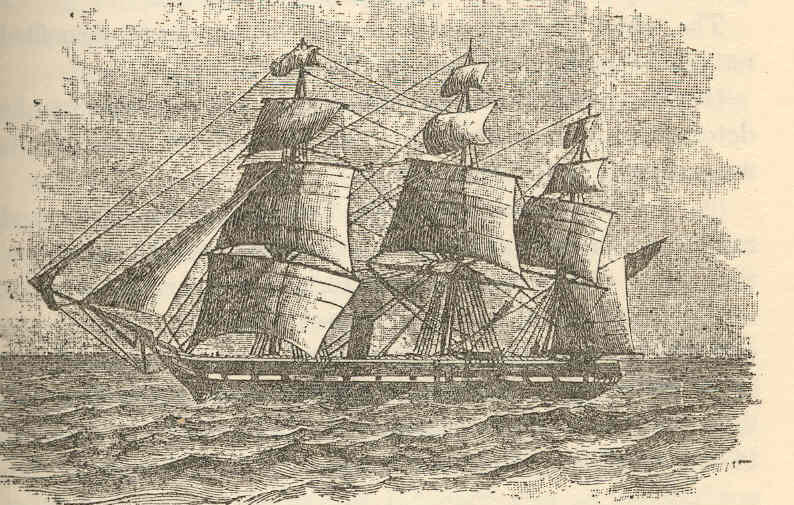
\includegraphics[width=0.55\linewidth]{images/book1/g8-challenger-sounding.jpg}

{\small السفينة \emph{تشالنجر} تستعد لسبر عمق \omterm{def:g2:water-on-earth:ocean}{المحيط}، 1872. نقش من تقارير
البعثة، أُعيد نشره في كتاب و.~أ.~هيردمان \emph{مؤسسو علم المحيطات}
(1923)؛ ملك عام، عبر ويكيميديا كومنز.}
% ledger: commons:challenger
\label{fig:g8:the-oceans:challenger}
\end{omfigure}

اليوم ترسم السفينة \omterm{def:g2:drawing-to-map:map}{خريطة} قاع \omterm{def:g2:water-on-earth:ocean}{البحر} بالصوت. فجهاز تحت بدنها يرسل نبضة
قصيرة من الصوت نحو الأسفل؛ فيرتد الصوت عن القاع ويعود صدى. والزمن الذي
يستغرقه الصدى يعطي العمق، مرة بعد مرة، بينما تواصل السفينة إبحارها. هذا هو
\emph{السونار}.
% ledger: nos:sonar

\begin{recall}
\omterm{def:g2:water-on-earth:salt-fresh}{الماء المالح} يغطي معظم الأرض، في \omterm{def:g2:water-on-earth:ocean}{محيط} عالمي واحد مقسَّم إلى محيطات وبحار
(\cref{ch:g2:water-on-earth}). وتتباعد \omterm{def:g7:plate-tectonics:plate}{الصفائح} عند الظهرات المحيطية، وتغوص
\omterm{def:g7:plate-tectonics:plate}{صفيحة} تحت أخرى عند الخنادق (\cref{ch:g7:plate-tectonics}). وفوق المحيطات تهب
الرياح في أحزمة كبرى: \omterm{def:g8:winds-global-circulation:global-winds}{الرياح التجارية}، \omterm{def:g8:winds-global-circulation:global-winds}{والرياح الغربية}، \omterm{def:g8:winds-global-circulation:global-winds}{والرياح الشرقية
القطبية}، يحرفها دوران الأرض (\cref{ch:g8:winds-global-circulation}).
\end{recall}

\section{قاع المحيط}

لو أمكن تصريف ماء المحيطات، لظهر \omterm{def:g1:landscapes-around-us:landscape}{منظر} طبيعي خفي كامل. فعلى طول \omterm{def:g1:landscapes-around-us:water}{السواحل}،
تمتد اليابسة تحت \omterm{def:g2:water-on-earth:ocean}{البحر} رفًّا قليل العمق لطيف الانحدار. ثم يهوي القاع على
منحدر شديد إلى \omterm{def:g1:landscapes-around-us:landform}{سهول} فسيحة مستوية، على عمق كيلومترات. وترتفع من هذه \omterm{def:g1:landscapes-around-us:landform}{السهول}
\omterm{def:g4:world-physical-map:range}{سلاسل جبلية}، وهنا وهناك تنزل خنادق ضيقة أعمق من أي شيء آخر على
الأرض.
% ledger: edin:challenger-stations

\begin{omfigure}
\begin{tikzpicture}[font=\footnotesize, >={Stealth[length=2mm]}]
  \fill[omSea] (0,0) rectangle (15.6,-4.2);
  \fill[omLithAlluv] (0,0.6) -- (1.2,0.15) -- (1.6,0) -- (3.4,-0.35)
    .. controls (3.9,-0.55) and (4.1,-2.6) .. (4.7,-3.1)
    -- (6.6,-3.35) -- (7.6,-3.1) -- (8.3,-2.2) -- (8.6,-1.7) -- (8.75,-1.9) -- (8.9,-1.65) -- (9.2,-2.3) -- (10.0,-3.15)
    -- (11.6,-3.4) -- (12.6,-3.45) -- (13.05,-4.1) -- (13.35,-3.0) -- (14.2,-0.9) -- (14.8,0.7) -- (15.6,1.3)
    -- (15.6,-4.6) -- (0,-4.6) -- cycle;
  \draw[black!70] (0,0.6) -- (1.2,0.15) -- (1.6,0) -- (3.4,-0.35)
    .. controls (3.9,-0.55) and (4.1,-2.6) .. (4.7,-3.1)
    -- (6.6,-3.35) -- (7.6,-3.1) -- (8.3,-2.2) -- (8.6,-1.7) -- (8.75,-1.9) -- (8.9,-1.65) -- (9.2,-2.3) -- (10.0,-3.15)
    -- (11.6,-3.4) -- (12.6,-3.45) -- (13.05,-4.1) -- (13.35,-3.0) -- (14.2,-0.9) -- (14.8,0.7) -- (15.6,1.3);
  \draw[omRiver] (1.55,0) -- (14.45,0);
  \node[anchor=south] at (8,0.05) {مستوى سطح البحر};
  \node[align=center] at (2.6,-0.85) {الرف\\القاري};
  \draw[->] (2.6,-0.55) -- (2.6,-0.25);
  \node[align=center, anchor=east] at (3.7,-2.0) {المنحدر\\القاري};
  \draw[->] (3.75,-2.0) -- (4.1,-1.9);
  \node[align=center] at (5.7,-2.6) {سهل سحيق};
  \node[align=center] at (8.75,-0.9) {ظهرة محيطية};
  \draw[->] (8.75,-1.15) -- (8.75,-1.55);
  \node[align=center] at (11.1,-2.6) {سهل سحيق};
  \node[align=center, anchor=west] at (13.5,-3.9) {خندق\\محيطي};
  \draw[->] (13.45,-3.9) -- (13.15,-3.9);
  \node[anchor=south] at (0.8,0.6) {قارة};
  \node[anchor=south east] at (14.7,1.0) {جبال};
\end{tikzpicture}

{\small أجزاء قاع \omterm{def:g2:water-on-earth:ocean}{المحيط}، من \omterm{def:g1:landscapes-around-us:water}{ساحل} إلى \omterm{def:g2:water-on-earth:ocean}{المحيط} المفتوح ثم إلى \omterm{def:g1:landscapes-around-us:water}{ساحل} آخر (رسم
تخطيطي: الأعماق والعروض ليست بمقياس رسم واحد).}
\label{fig:g8:the-oceans:sketch}
\end{omfigure}

\begin{definition}[أجزاء قاع المحيط]\label{def:g8:the-oceans:seafloor}
\begin{itemize}
  \item \emph{الرف القاري}\index{رف قاري} هو حافة \omterm{def:g3:continents-and-oceans:continent}{القارة} تحت \omterm{def:g2:water-on-earth:ocean}{البحر}،
        وهي قليلة العمق ولطيفة الانحدار.
  \item \emph{المنحدر القاري}\index{منحدر قاري} هو المنحدر الشديد الذي
        يهبط من الرف إلى قاع \omterm{def:g2:water-on-earth:ocean}{المحيط} العميق.
  \item \emph{السهل السحيق}\index{سهل سحيق} جزء فسيح من قاع \omterm{def:g2:water-on-earth:ocean}{المحيط}، مستوٍ
        جدًا وعميق.
  \item \emph{الظهرة المحيطية}\index{ظهرة محيطية} سلسلة طويلة من
        \omterm{def:g1:landscapes-around-us:landform}{الجبال} المغمورة ترتفع من \omterm{def:g1:landscapes-around-us:landform}{السهول} السحيقة.
  \item \emph{الخندق المحيطي}\index{خندق محيطي} منخفض طويل ضيق
        عميق جدًا في قاع \omterm{def:g2:water-on-earth:ocean}{المحيط}، كثيرًا ما يقع بجوار سلسلة من
        \omterm{def:g1:landscapes-around-us:landform}{الجبال} أو الجزر البركانية.
\end{itemize}
\end{definition}
% ledger: edin:challenger-stations, usgs:trench-depth

يبلغ متوسط عمق \omterm{def:g2:water-on-earth:ocean}{المحيط} نحو \qty{3700}{m}، أي قرابة نصف \omterm{def:g4:world-physical-map:altitude}{ارتفاع} أعلى \omterm{def:g1:landscapes-around-us:landform}{جبل} على
اليابسة. وأعمق نقطة فيه، غور تشالنجر في خندق ماريانا في \omterm{def:g2:water-on-earth:ocean}{المحيط} الهادئ،
تقع على عمق يقارب \qty{11000}{m} تحت
السطح.
% ledger: nos:ocean-depth, usgs:trench-depth, tht:everest


\begin{method}[قراءة مقطع جانبي لقاع المحيط]
\begin{enumerate}
  \item اقرأ المحورين: المسافة أفقيًا، \omterm{def:g4:world-physical-map:altitude}{والارتفاع} أو العمق رأسيًا،
        والمبالغة الرأسية.
  \item جد \omterm{def:g4:world-physical-map:altitude}{مستوى سطح البحر} (\omterm{def:g4:world-physical-map:altitude}{الارتفاع} 0) \omterm{def:g1:landscapes-around-us:water}{والسواحل} حيث يقطعه
        المقطع.
  \item تتبّع القاع انطلاقًا من \omterm{def:g1:landscapes-around-us:water}{ساحل}: الرف قليل العمق، ثم المنحدر الشديد،
        ثم \omterm{def:g1:landscapes-around-us:landform}{السهول} العميقة المستوية.
  \item ابحث عما يرتفع فوق \omterm{def:g1:landscapes-around-us:landform}{السهول} (ظهرة) أو ينخفض تحتها
        (خندق)، واقرأ عمقه.
\end{enumerate}
\end{method}

\begin{example}[عبر جنوب المحيط الأطلسي]
في المقطع العلوي، بعد \omterm{def:g1:landscapes-around-us:water}{ساحل} أمريكا الجنوبية، يهبط القاع إلى عمق يزيد على
\qty{3000}{m} في أقل من \qty{300}{km}. وتملأ \omterm{def:g1:landscapes-around-us:landform}{سهول} سحيقة، على عمق بين
\qty{3500}{m} و\qty{5000}{m}، معظم العرض. وفي منتصف الطريق، على بعد نحو
\qty{4400}{km} على طول المقطع، ترتفع ظهرة وسط الأطلسي إلى نحو \qty{2300}{m}
تحت السطح: أي أكثر من \qty{2000}{m} فوق \omterm{def:g1:landscapes-around-us:landform}{السهول}، \omterm{def:g4:world-physical-map:range}{سلسلة جبلية} مخبوءة تحت \omterm{def:g2:water-on-earth:ocean}{البحر}.
ثم تزداد \omterm{def:g1:landscapes-around-us:landform}{السهول} عمقًا من جديد إلى أكثر من \qty{5000}{m} قبل أن يصعد القاع نحو
إفريقيا.
\end{example}
% ledger: data:etopo1 (figdata/grade-8/seafloor_profile.py: ridge crest -2329 m at 4407 km; deepest -5295 m)

\begin{omfigure}
\begin{tikzpicture}
\begin{axis}[omsection, scale only axis, width=14cm, height=3.6cm, xmin=0, xmax=7569,
  ymin=-6000, ymax=1500, ytick={-6000,-4000,-2000,0}, xtick={0,1000,...,7000},
  xlabel={\foreignlanguage{arabic}{المسافة على خط العرض \babelsublr{30.5\textdegree} جنوبًا، انطلاقًا من \babelsublr{59.5\textdegree} غربًا \babelsublr{(km)}}}, ylabel={\foreignlanguage{arabic}{الارتفاع \babelsublr{(m)}}},
  tick label style={font=\scriptsize}, label style={font=\small},
  yticklabel style={/pgf/number format/1000 sep={\,}}, xticklabel style={/pgf/number format/1000 sep={\,}},
  axis background/.style={fill=white}, clip=true]
  \fill[omSea] (axis cs:0,-6000) rectangle (axis cs:7569,0);
  \addplot[fill=omLithAlluv, draw=black!70, line width=0.5pt] table[x=km, y=elev_m] {figdata/out/grade-8-seafloor_profile-atlantic-rock.dat};
  \node[font=\scriptsize, align=center, fill=white, inner sep=1pt] at (axis cs:4407,-900) {ظهرة وسط الأطلسي};
  \draw[-{Stealth[length=1.5mm]}] (axis cs:4407,-1250) -- (axis cs:4407,-2150);
  \node[font=\scriptsize] at (axis cs:2500,-5300) {سهل سحيق};
  \node[font=\scriptsize] at (axis cs:6200,-5600) {سهل سحيق};
  \node[font=\scriptsize, anchor=south west] at (axis cs:30,350) {أمريكا الجنوبية};
  \node[font=\scriptsize, anchor=south east] at (axis cs:7380,350) {إفريقيا};
  \node[anchor=north] at (rel axis cs:0.75,0.97) {\omve{260}};
\end{axis}
\end{tikzpicture}

\medskip
\begin{tikzpicture}
\begin{axis}[omsection, scale only axis, width=7cm, height=3.6cm, xmin=0, xmax=3020,
  ymin=-6000, ymax=4500, ytick={-6000,-4000,-2000,0,2000,4000}, xtick={0,1000,2000,3000},
  xlabel={\foreignlanguage{arabic}{المسافة على خط العرض \babelsublr{20.5\textdegree} جنوبًا \babelsublr{(km)}}}, ylabel={\foreignlanguage{arabic}{الارتفاع \babelsublr{(m)}}},
  tick label style={font=\scriptsize}, label style={font=\small},
  yticklabel style={/pgf/number format/1000 sep={\,}}, xticklabel style={/pgf/number format/1000 sep={\,}},
  axis background/.style={fill=white}, clip=true]
  \fill[omSea] (axis cs:0,-6000) rectangle (axis cs:3020,0);
  \addplot[fill=omLithAlluv, draw=black!70, line width=0.5pt] table[x=km, y=elev_m] {figdata/out/grade-8-seafloor_profile-pacific-rock.dat};
  \node[font=\scriptsize, align=center, fill=white, inner sep=1pt] at (axis cs:1300,1600) {خندق بيرو-تشيلي};
  \draw[-{Stealth[length=1.5mm]}] (axis cs:1750,1150) -- (axis cs:1870,-5000);
  \node[font=\scriptsize, anchor=west] at (axis cs:2600,3500) {الأنديز};
  \node[font=\scriptsize] at (axis cs:700,-5300) {سهل سحيق};
  \node[anchor=north west] at (rel axis cs:0.01,0.98) {\omve{148}};
\end{axis}
\end{tikzpicture}

{\small مقطعان جانبيان حقيقيان لقاع \omterm{def:g2:water-on-earth:ocean}{المحيط}، من تضاريس ETOPO1 مقروءة عند كل
درجة من \omterm{def:g6:latitude-longitude:longitude}{خطوط الطول}. في الأعلى: عبر جنوب الأطلسي، من أمريكا الجنوبية إلى
إفريقيا. وفي الأسفل: عبر حافة \omterm{def:g2:water-on-earth:ocean}{المحيط} الهادئ عند أمريكا الجنوبية. وقد مُطَّت
الارتفاعات 260 مرة و148 مرة مقارنةً بالمسافات (\emph{المبالغة الرأسية})، وإلا
لبدا \omterm{def:g2:water-on-earth:ocean}{المحيط} رقيقًا كورقة؛ ومع نقطة واحدة عند كل درجة، يبدو الخندق الضيق أقل
عمقًا مما هو في الحقيقة.}
% ledger: data:etopo1, earth:Rmean (figdata/grade-8/seafloor_profile.py)
\label{fig:g8:the-oceans:profiles}
\end{omfigure}


\section{الماء المالح}

طعم ماء \omterm{def:g2:water-on-earth:ocean}{البحر} مالح لأن فيه أملاحًا ذائبة. ومعظمها يأتي من \omterm{def:g3:stones-pebbles-sand:rock}{صخور} \omterm{def:g3:continents-and-oceans:continent}{القارات}:
\omterm{def:g4:clouds-rain-snow:precipitation}{فالمطر} يبري \omterm{def:g3:stones-pebbles-sand:rock}{الصخور} ببطء، \omterm{def:g1:landscapes-around-us:water}{والأنهار} تحمل أملاحها الذائبة إلى \omterm{def:g2:water-on-earth:ocean}{البحر}. وبعضها
يأتي من ينابيع حارة في قاع \omterm{def:g2:water-on-earth:ocean}{المحيط}.
% ledger: nos:salinity-varies

\begin{definition}[الملوحة]\label{def:g8:the-oceans:salinity}
\emph{ملوحة}\index{ملوحة} ماء \omterm{def:g2:water-on-earth:ocean}{البحر} هي كتلة الأملاح الذائبة في كيلوغرام من ماء
\omterm{def:g2:water-on-earth:ocean}{البحر}. ومتوسطها نحو \qty{35}{g} في الكيلوغرام: أي إن \qty{3.5}{\%} من كتلة
ماء \omterm{def:g2:water-on-earth:ocean}{البحر} ملح.
\end{definition}
% ledger: nos:salinity-varies

ليست \omterm{def:g8:the-oceans:salinity}{الملوحة} واحدة في كل مكان. فحين يتبخر ماء \omterm{def:g2:water-on-earth:ocean}{البحر}، يرحل الماء وتبقى
الأملاح: فحيث تكون الشمس قوية \omterm{def:g4:clouds-rain-snow:precipitation}{والمطر} نادرًا، يصير \omterm{def:g2:water-on-earth:ocean}{البحر} أكثر \omterm{def:g8:the-oceans:salinity}{ملوحة}. وحيث
يهطل \omterm{def:g4:clouds-rain-snow:precipitation}{مطر} كثير، أو حيث يصب \omterm{def:g1:landscapes-around-us:water}{نهر} كبير، يكون \omterm{def:g2:water-on-earth:ocean}{البحر} أقل \omterm{def:g8:the-oceans:salinity}{ملوحة}. وحين يتجمد ماء
\omterm{def:g2:water-on-earth:ocean}{البحر} فيصير جليدًا بحريًا، يبقى الملح في الماء \omterm{def:g2:water-on-earth:ocean}{المحيط} به، فيصير هو أيضًا
أكثر \omterm{def:g8:the-oceans:salinity}{ملوحة}. وعلى العموم، تكون \omterm{def:g8:the-oceans:salinity}{الملوحة} منخفضة قرب \omterm{def:g3:continents-and-oceans:equator}{خط الاستواء}، حيث يكثر \omterm{def:g4:clouds-rain-snow:precipitation}{المطر}،
وقرب \omterm{def:g3:continents-and-oceans:poles}{القطبين}؛ وتبلغ أعلاها في العروض الوسطى، تحت الأحزمة الجافة قرب
\ang{30}.
% ledger: nos:salinity-varies, nos:sea-ice-salt, mo:three-cells

\begin{omfigure}
\begin{tikzpicture}[font=\footnotesize, >={Stealth[length=2mm]}]
  \fill[omSea] (0,0) rectangle (13,-1.6);
  \draw[omRiver, line width=0.8pt] (0,0) -- (13,0);
  % left: dry belt, evaporation
  \fill[yellow!80!orange] (1.2,3.0) circle (0.35);
  \foreach \x in {1.0,1.8,2.6,3.4} \draw[->, black!50, line width=0.9pt, decorate, decoration={snake, amplitude=0.6mm, segment length=3mm}] (\x,0.15) -- (\x,1.6);
  \node[align=center] at (2.3,2.2) {تبخر قوي\\ومطر قليل};
  \node[align=center, fill=white, inner sep=1.5pt] at (2.3,-0.8) {\textbf{أكثر ملوحة}};
  % middle: rain
  \fill[black!20] (5.2,2.9) ellipse [x radius=1.3, y radius=0.4];
  \foreach \x in {4.4,4.8,...,6.0} \draw[omRiver] (\x,2.45) -- (\x-0.2,0.25);
  \node[align=center, fill=white, inner sep=1.5pt] at (5.2,-0.8) {\textbf{أقل ملوحة}};
  \node at (5.2,3.55) {مطر غزير};
  % right: river mouth and sea ice
  \fill[omLithAlluv] (7.4,0) -- (9.6,0) -- (9.6,0.6) -- (7.4,0.35) -- cycle;
  \draw[omRiver, line width=2pt, ->] (9.4,0.45) -- (7.9,0.2);
  \node[anchor=south] at (8.6,0.65) {نهر};
  \node[align=center, fill=white, inner sep=1.5pt] at (8.6,-0.8) {\textbf{أقل ملوحة}};
  \fill[white, draw=omCold] (10.6,0.25) -- (12.6,0.25) -- (12.4,-0.25) -- (10.8,-0.25) -- cycle;
  \node[anchor=south] at (11.6,0.3) {يتكون الجليد البحري};
  \node[align=center, fill=white, inner sep=1.5pt] at (11.6,-0.95) {\textbf{أكثر ملوحة}\\(يبقى الملح في الماء)};
\end{tikzpicture}

{\small ما الذي يغير \omterm{def:g8:the-oceans:salinity}{ملوحة} \omterm{def:g2:water-on-earth:ocean}{البحر}: التبخر والتجمد يتركان الأملاح وراءهما؛
\omterm{def:g4:clouds-rain-snow:precipitation}{والمطر} \omterm{def:g1:landscapes-around-us:water}{والأنهار} تضيف ماءً عذبًا.}
% ledger: nos:salinity-varies, nos:sea-ice-salt
\label{fig:g8:the-oceans:salinity}
\end{omfigure}

\begin{omfigure}
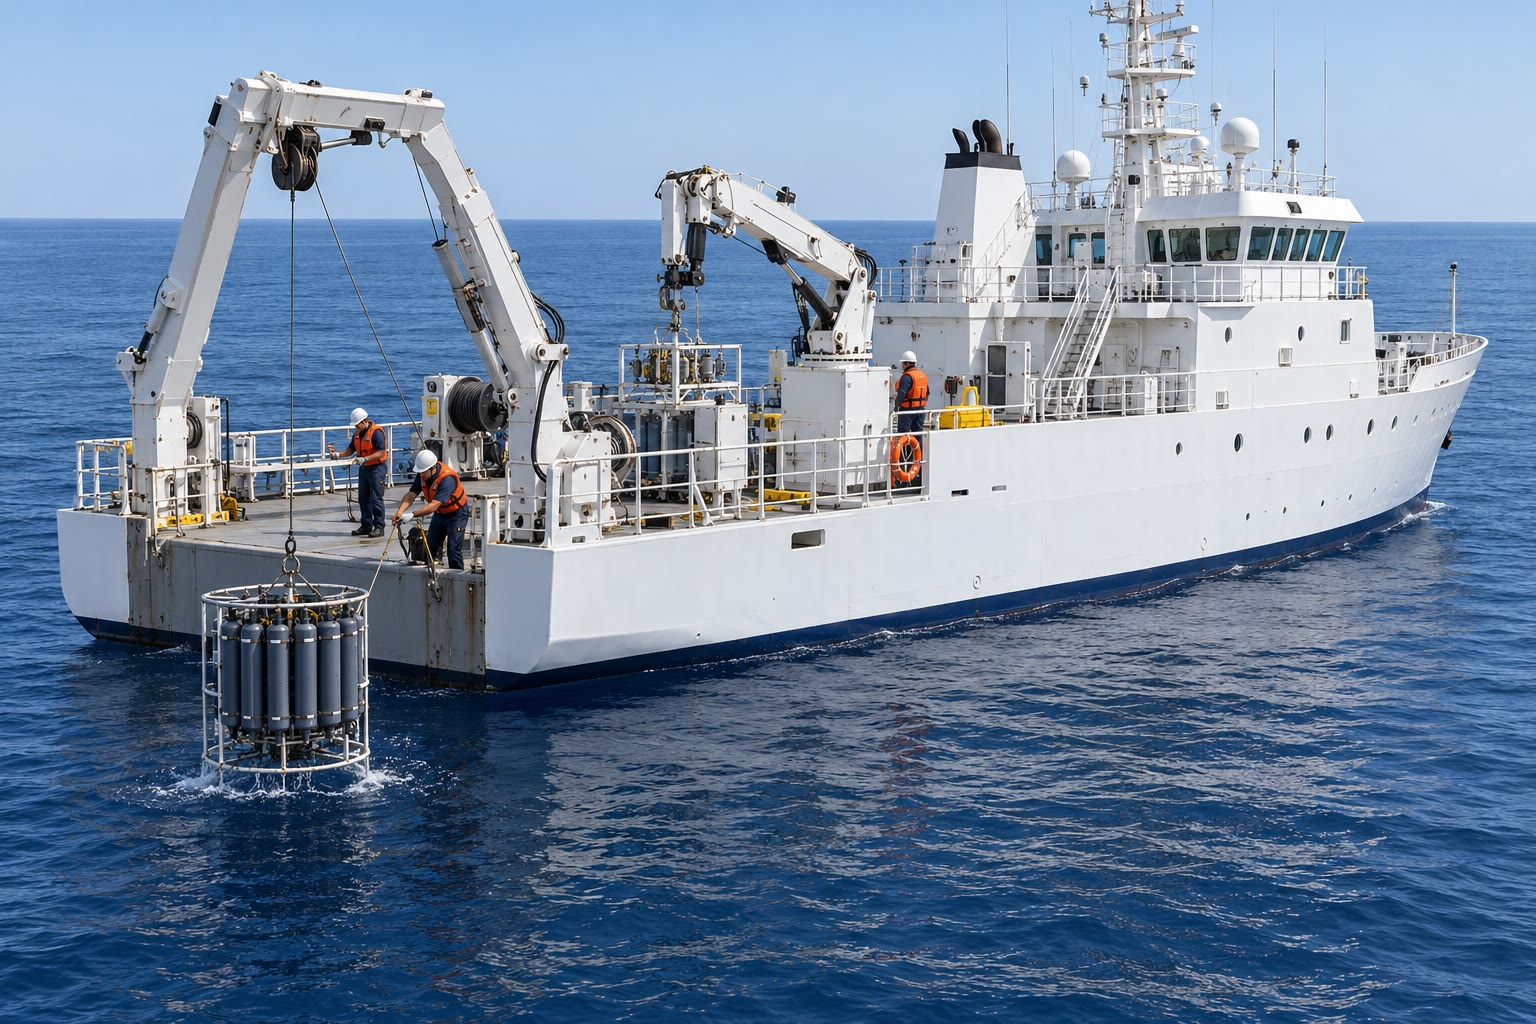
\includegraphics[width=0.58\linewidth]{images/book1/ai/g8-research-ship.jpg}

{\small سفينة أبحاث تُنزل في \omterm{def:g2:water-on-earth:ocean}{البحر} إطارًا من قوارير أخذ العينات، لتعيد ماءً
من الأعماق وتقيس ملوحته ودرجة حرارته (رسم توضيحي مولَّد بالذكاء الاصطناعي
لمشهد عام).}
\label{fig:g8:the-oceans:ship}
\end{omfigure}

\section{التيارات السطحية}

\omterm{def:g2:water-on-earth:ocean}{المحيط} لا يسكن أبدًا. فالرياح تجرّ سطحه وتحرك الماء: \omterm{def:g8:winds-global-circulation:global-winds}{الرياح التجارية}
المنتظمة تدفعه نحو الغرب قرب \omterm{def:g3:continents-and-oceans:equator}{خط الاستواء}، \omterm{def:g8:winds-global-circulation:global-winds}{والرياح الغربية} تدفعه نحو الشرق
في العروض الوسطى. ومثل الرياح، ينحرف الماء المتحرك بفعل دوران الأرض: إلى
اليمين في \omterm{def:g3:continents-and-oceans:equator}{نصف الكرة الشمالي}، وإلى اليسار في \omterm{def:g3:continents-and-oceans:equator}{نصف الكرة
الجنوبي}.
% ledger: nos:gyres

\begin{definition}[التيار المحيطي والدوامة المحيطية]\label{def:g8:the-oceans:current}
\emph{التيار المحيطي}\index{تيار محيطي} حركة منتظمة لماء \omterm{def:g2:water-on-earth:ocean}{البحر} في اتجاه
واحد، \omterm{def:g1:landscapes-around-us:water}{كنهر} في \omterm{def:g2:water-on-earth:ocean}{المحيط}. و\emph{الدوامة المحيطية}\index{دوامة محيطية} حلقة
كبيرة جدًا من التيارات المحيطية تدور حول حوض
محيطي.
\end{definition}
% ledger: nos:gyre-def, nos:gyres
\phantomsection\label{def:g8:the-oceans:gyre}

هناك خمس \omterm{def:g8:the-oceans:current}{دوامات محيطية} كبرى: في شمال الأطلسي وجنوبه، وفي شمال الهادئ
وجنوبه، وفي \omterm{def:g2:water-on-earth:ocean}{المحيط} الهندي. \omterm{def:g8:the-oceans:current}{ودوامات} \omterm{def:g3:continents-and-oceans:equator}{نصف الكرة الشمالي} تدور مع اتجاه عقارب
الساعة، \omterm{def:g8:the-oceans:current}{ودوامات} \omterm{def:g3:continents-and-oceans:equator}{نصف الكرة الجنوبي} عكسه. وعلى الجانب الغربي من كل \omterm{def:g2:water-on-earth:ocean}{محيط}،
يكون تيار \omterm{def:g8:the-oceans:current}{الدوامة} ضيقًا سريعًا؛ وعلى الجانب الشرقي، عريضًا
بطيئًا.
% ledger: nos:gyres

\begin{inthelab}[دوامة في صحن]
داخل البيت، املأ صحنًا مستديرًا كبيرًا بالماء وانثر رشة من الفلفل على
السطح. انفخ برفق وبانتظام عبر الصحن بماصّة، دائمًا في الاتجاه نفسه، قرب
الحافة. وراقب الفلفل: فالماء القريب من السطح يبدأ يتحرك مع نفَسك، وسرعان
ما يدور السطح كله في حلقة حول الصحن.
\end{inthelab}

\begin{omfigure}
\begin{tikzpicture}
\begin{axis}[ommap, width=\linewidth, xmin=-180, xmax=180, ymin=-65, ymax=70,
  xtick={-180,-120,...,180}, ytick={-60,-30,0,30,60},
  xticklabels={$180^\circ$,\foreignlanguage{arabic}{$120^\circ$ غ},\foreignlanguage{arabic}{$60^\circ$ غ},$0^\circ$,\foreignlanguage{arabic}{$60^\circ$ ق},\foreignlanguage{arabic}{$120^\circ$ ق},$180^\circ$},
  yticklabels={\foreignlanguage{arabic}{$60^\circ$ ج},\foreignlanguage{arabic}{$30^\circ$ ج},$0^\circ$,\foreignlanguage{arabic}{$30^\circ$ ش},\foreignlanguage{arabic}{$60^\circ$ ش}},
  tick label style={font=\scriptsize}]
  \addplot[fill=omLithAlluv, draw=black!45, line width=0.2pt] table {figdata/out/shared-geo-land.dat};
  \addplot[omWarm, line width=1.3pt] table {figdata/out/grade-8-ocean_currents-gyres-warm.dat};
  \addplot[omCold, line width=1.3pt] table {figdata/out/grade-8-ocean_currents-gyres-cold.dat};
  \addplot[quiver={u=\thisrow{u}, v=\thisrow{v}}, -{Stealth[length=2.6mm, width=2.2mm]}, omWarm, line width=1.3pt]
    table[x=lon, y=lat] {figdata/out/grade-8-ocean_currents-heads-warm.dat};
  \addplot[quiver={u=\thisrow{u}, v=\thisrow{v}}, -{Stealth[length=2.6mm, width=2.2mm]}, omCold, line width=1.3pt]
    table[x=lon, y=lat] {figdata/out/grade-8-ocean_currents-heads-cold.dat};
  \node[font=\scriptsize\bfseries, fill=white, inner sep=1pt, anchor=east] at (axis cs:-72,40) {تيار الخليج};
  \node[font=\scriptsize\bfseries, fill=white, inner sep=1pt, anchor=west] at (axis cs:-12,25) {تيار الكناري};
\end{axis}
\end{tikzpicture}

{\small \omterm{def:g8:the-oceans:current}{الدوامات} الخمس الكبرى، مبسَّطة: مع اتجاه عقارب الساعة في \omterm{def:g3:continents-and-oceans:equator}{نصف الكرة
الشمالي}، وعكسه في الجنوبي. بالأحمر: التيارات الدافئة، الآتية من المناطق
المدارية؛ وبالأزرق: التيارات الباردة، الآتية من عروض أعلى. ويحدّ دوامةَ شمال
الأطلسي تيارُ الخليج من الغرب وتيارُ الكناري من
الشرق.}
% ledger: nos:gyres, data:ne-land (figdata/grade-8/ocean_currents.py)
\label{fig:g8:the-oceans:gyres}
\end{omfigure}

أشهر هذه التيارات تيار الخليج. فهو يغادر خليج المكسيك، ويجري شمالًا على طول
\omterm{def:g1:landscapes-around-us:water}{ساحل} فلوريدا، ثم ينعطف شرقًا قبالة كارولاينا الشمالية ويعبر الأطلسي نحو
الشمال الشرقي. ويتحرك ماؤه الدافئ بمتوسط نحو \qty{6.4}{km} في الساعة، وتبلغ
سرعته عند السطح نحو \qty{9}{km} في الساعة، ويحمل من الماء أكثر مما تحمله
\omterm{def:g1:landscapes-around-us:water}{أنهار} العالم كلها مجتمعة. وهو يُبقي \omterm{def:g1:landscapes-around-us:water}{الساحل} الشرقي لفلوريدا أدفأ في الشتاء
ويجلب هواءً معتدلًا إلى غرب أوروبا.
% ledger: nos:gulf-stream, nos:gyres

\begin{omfigure}
\begin{minipage}[c]{0.5\linewidth}\centering
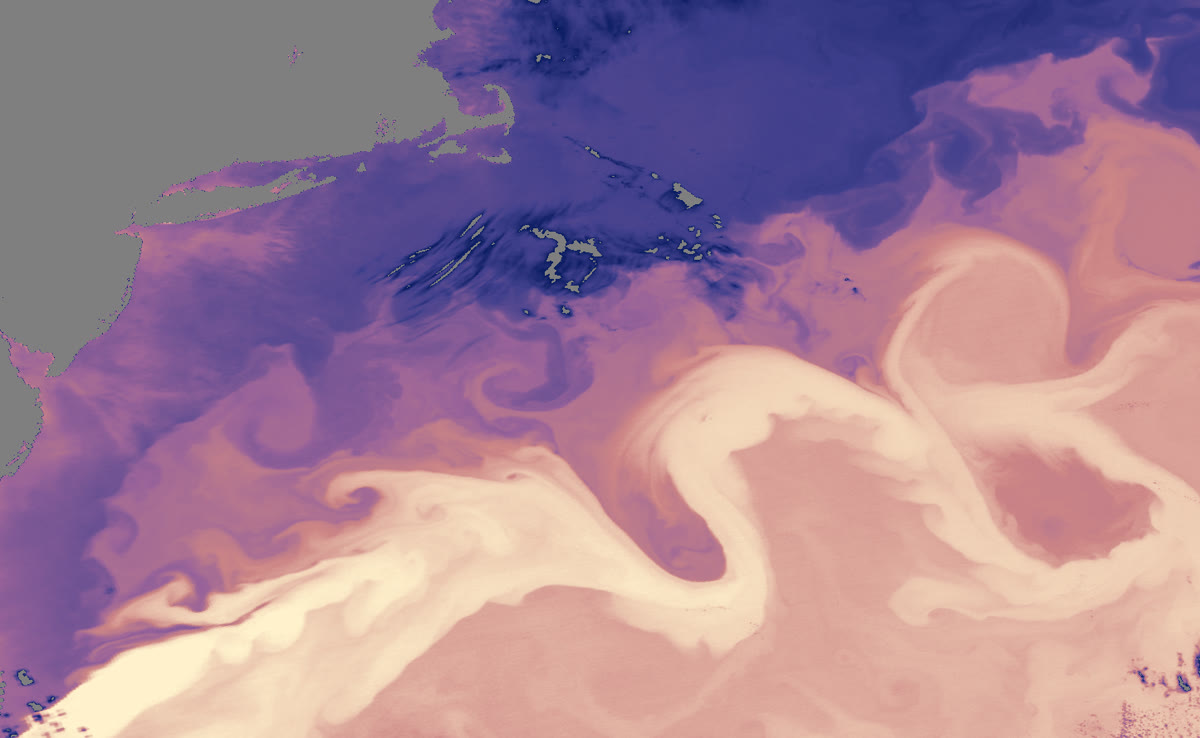
\includegraphics[width=\linewidth]{images/book1/g8-gulf-stream-sst.jpg}
\end{minipage}\hfill
\begin{minipage}[c]{0.46\linewidth}\raggedright
{\small درجة حرارة سطح \omterm{def:g2:water-on-earth:ocean}{البحر} قبالة \omterm{def:g1:landscapes-around-us:water}{الساحل} الشرقي لأمريكا الشمالية، كما قاسها
القمر الصناعي أكوا التابع لناسا في 18~أبريل 2005. تيار الخليج هو شريط الماء
الدافئ (الألوان الفاتحة، حتى نحو \qty{23}{\degreeCelsius}) الذي يتلوى من أسفل
اليسار نحو اليمين، بين مياه أبرد (داكنة، حتى نحو
\qty{-1}{\degreeCelsius})؛ واليابسة رمادية. ناسا (ملك عام، عبر ويكيميديا
كومنز).}
\end{minipage}
% ledger: commons:gulf-sst
\label{fig:g8:the-oceans:gulf}
\end{omfigure}


\section{التيارات العميقة وحرارة المحيط}

الرياح تحرك التيارات السطحية. وفي الأسفل البعيد، في الظلام البارد \omterm{def:g2:water-on-earth:ocean}{للمحيط}
العميق، يتحرك الماء أيضًا، لكن ببطء أشد بكثير. ففي أقصى شمال الأطلسي، يعطي
الماء الدافئ الذي جلبه تيار الخليج حرارته للهواء البارد؛ فيبرد، ويزداد \omterm{def:g8:the-oceans:salinity}{ملوحة}
حين يتكون الجليد البحري، فيصير أكثف ويغوص إلى القاع. ويزحف هذا الماء البارد
المالح جنوبًا على طول قاع \omterm{def:g2:water-on-earth:ocean}{المحيط}، حتى القارة القطبية الجنوبية، ثم إلى
المحيطين الهندي والهادئ، حيث يصعد ببطء ويعود إلى السطح. وقد تستغرق قطرة
الماء نحو \num{1000} سنة لتدور مرة واحدة حول هذه الحلقة الكبرى، أي
\emph{الحزام الناقل المحيطي العالمي}.
% ledger: nos:conveyor, nos:sea-ice-salt

\begin{omfigure}
\begin{tikzpicture}
\begin{axis}[ommap, width=\linewidth, xmin=-180, xmax=180, ymin=-65, ymax=70,
  xtick={-180,-120,...,180}, ytick={-60,-30,0,30,60},
  xticklabels={$180^\circ$,\foreignlanguage{arabic}{$120^\circ$ غ},\foreignlanguage{arabic}{$60^\circ$ غ},$0^\circ$,\foreignlanguage{arabic}{$60^\circ$ ق},\foreignlanguage{arabic}{$120^\circ$ ق},$180^\circ$},
  yticklabels={\foreignlanguage{arabic}{$60^\circ$ ج},\foreignlanguage{arabic}{$30^\circ$ ج},$0^\circ$,\foreignlanguage{arabic}{$30^\circ$ ش},\foreignlanguage{arabic}{$60^\circ$ ش}},
  tick label style={font=\scriptsize}]
  \addplot[fill=omLithAlluv, draw=black!45, line width=0.2pt] table {figdata/out/shared-geo-land.dat};
  \addplot[omWarm, line width=1.3pt] table {figdata/out/grade-8-conveyor-surface.dat};
  \addplot[omCold, line width=1.3pt, dashed] table {figdata/out/grade-8-conveyor-deep.dat};
  \addplot[quiver={u=\thisrow{u}, v=\thisrow{v}}, -{Stealth[length=2.6mm, width=2.2mm]}, omWarm, line width=1.3pt]
    table[x=lon, y=lat] {figdata/out/grade-8-conveyor-heads-surface.dat};
  \addplot[quiver={u=\thisrow{u}, v=\thisrow{v}}, -{Stealth[length=2.6mm, width=2.2mm]}, omCold, line width=1.3pt]
    table[x=lon, y=lat] {figdata/out/grade-8-conveyor-heads-deep.dat};
  \node[font=\scriptsize\bfseries, fill=white, inner sep=1pt, anchor=west] at (axis cs:4,64) {يغوص};
  \node[font=\scriptsize\bfseries, fill=white, inner sep=1pt, anchor=south] at (axis cs:163,11) {يصعد};
\end{axis}
\end{tikzpicture}

{\small الحزام الناقل المحيطي العالمي، مبسَّطًا في حلقة واحدة (رسم تخطيطي).
بالأحمر: الماء الدافئ عند السطح؛ وبالأزرق المتقطع: الماء البارد المالح الزاحف
على طول قاع \omterm{def:g2:water-on-earth:ocean}{المحيط} العميق. يغوص الماء في أقصى شمال الأطلسي، بين غرينلاند
والنرويج، ويصعد في \omterm{def:g2:water-on-earth:ocean}{المحيط} الهادئ (وفي \omterm{def:g2:water-on-earth:ocean}{المحيط} الهندي، وهو غير
مرسوم).}
% ledger: nos:conveyor, data:ne-land (figdata/grade-8/conveyor.py)
\end{omfigure}

\begin{example}[ما مدى بطء الماء العميق؟]\label{ex:g8:the-oceans:deep-speed}
يبلغ طول الحلقة المرسومة على \omterm{def:g2:drawing-to-map:map}{الخريطة} نحو \qty{70000}{km}. فإذا استغرقت قطرة
الماء نحو \num{1000} سنة لتدور حولها، فهي تتحرك في المتوسط نحو
$\num{70000} \div \num{1000} = \qty{70}{km}$ في السنة، أي نحو
\qty{200}{m} في اليوم. أما تيار الخليج، بسرعة \qty{6.4}{km} في الساعة، فيقطع
نحو \qty{150}{km} في اليوم: فهو يقطع في نحو 11 ساعة ما يقطعه الماء العميق في
سنة كاملة.
% ledger: nos:conveyor, nos:gulf-stream, earth:Rmean (loop length and speeds computed in figdata/grade-8/conveyor.py)
\end{example}

تنقل التيارات السطحية والعميقة معًا الحرارة: فالماء الدافئ يتدفق من المناطق
المدارية نحو \omterm{def:g3:continents-and-oceans:poles}{القطبين}، والماء البارد يعود نحو \omterm{def:g3:continents-and-oceans:equator}{خط الاستواء}. ومثل الرياح، يعادل
\omterm{def:g2:water-on-earth:ocean}{المحيط} التسخين غير المتساوي للأرض بالشمس.
% ledger: nos:conveyor, nos:gulf-stream, mo:global-circ

\section{تمارين}

\begin{exercise}[$\star$]\label{exo:g8:the-oceans:1}
رتّب أجزاء قاع \omterm{def:g2:water-on-earth:ocean}{المحيط} هذه بالترتيب الذي تصادفها به غواصة تغادر ساحلًا
نحو وسط الأطلسي: \omterm{def:g8:the-oceans:seafloor}{سهل سحيق}؛ \omterm{def:g8:the-oceans:seafloor}{منحدر قاري}؛ \omterm{def:g8:the-oceans:seafloor}{ظهرة محيطية}؛ \omterm{def:g8:the-oceans:seafloor}{رف
قاري}.
\end{exercise}

\begin{exercise}[$\star$]\label{exo:g8:the-oceans:2}
صواب أم خطأ؟ صحّح الجمل الخاطئة. (أ) يبلغ متوسط عمق \omterm{def:g2:water-on-earth:ocean}{المحيط} نحو
\qty{37}{km}. (ب) تدور \omterm{def:g8:the-oceans:current}{دوامات} \omterm{def:g3:continents-and-oceans:equator}{نصف الكرة الشمالي} مع اتجاه عقارب الساعة. (ج)
التبخر يجعل ماء \omterm{def:g2:water-on-earth:ocean}{البحر} أقل \omterm{def:g8:the-oceans:salinity}{ملوحة}. (د) تيار الخليج تيار
دافئ.
\end{exercise}

\begin{exercise}[$\star$]\label{exo:g8:the-oceans:3}
أعطِ الكلمة المناسبة لكل وصف: (أ) سلسلة طويلة من \omterm{def:g1:landscapes-around-us:landform}{الجبال} تحت \omterm{def:g2:water-on-earth:ocean}{البحر}؛ (ب)
كتلة الملح في كيلوغرام من ماء \omterm{def:g2:water-on-earth:ocean}{البحر}؛ (ج) حلقة كبيرة جدًا من \omterm{def:g8:the-oceans:current}{التيارات
المحيطية}؛ (د) منخفض طويل ضيق عميق جدًا في قاع
\omterm{def:g2:water-on-earth:ocean}{المحيط}.
\end{exercise}

\begin{exercise}[$\star$]\label{exo:g8:the-oceans:4}
على \omterm{def:g2:drawing-to-map:map}{خريطة} \omterm{def:g8:the-oceans:current}{الدوامات}: (أ) في أي اتجاه تدور \omterm{def:g8:the-oceans:current}{دوامة} جنوب الأطلسي؟ (ب) سمِّ تيارًا
دافئًا وتيارًا باردًا في شمال الأطلسي. (ج) ما الرياح التي تدفع الماء نحو
الغرب قرب \omterm{def:g3:continents-and-oceans:equator}{خط الاستواء}؟
\end{exercise}

\begin{exercise}[$\star\star$]\label{exo:g8:the-oceans:5}
عينة من \qty{1}{kg} من ماء \omterm{def:g2:water-on-earth:ocean}{البحر} تحتوي على \qty{35}{g} من الأملاح. (أ)
ما النسبة المئوية للملح من كتلتها؟ (ب) كم غرامًا من الأملاح في
\qty{20}{kg} من هذا الماء؟ (ج) كم كيلوغرامًا من ماء \omterm{def:g2:water-on-earth:ocean}{البحر} يحتوي على
\qty{1}{kg} من الأملاح؟
\end{exercise}

\begin{exercise}[$\star\star$]\label{exo:g8:the-oceans:6}
يرسل سونار سفينة نبضة صوتية نحو الأسفل مباشرة. فيعود الصدى بعد
\qty{6}{s}. ويقطع الصوت في ماء \omterm{def:g2:water-on-earth:ocean}{البحر} نحو \qty{1500}{m} في كل ثانية. (أ) ما
المسافة التي يقطعها الصوت في \qty{6}{s}؟ (ب) لماذا لا يساوي العمق إلا نصف
هذه المسافة؟ (ج) ما العمق؟ (د) فوق أي جزء من قاع \omterm{def:g2:water-on-earth:ocean}{المحيط} قد تكون
السفينة؟
\end{exercise}

\begin{exercise}[$\star\star$]\label{exo:g8:the-oceans:7}
استعمل المقطع الجانبي عبر جنوب الأطلسي. (أ) ما عمق \omterm{def:g1:landscapes-around-us:landform}{السهول} السحيقة تقريبًا؟
(ب) على أي مسافة على طول المقطع تقع قمة ظهرة وسط الأطلسي، وما عمقها؟
(ج) بكم مترًا ترتفع الظهرة فوق \omterm{def:g1:landscapes-around-us:landform}{السهول}؟ (د) لماذا يحتاج المقطع إلى مبالغة
رأسية؟
\end{exercise}

\begin{exercise}[$\star\star$]\label{exo:g8:the-oceans:8}
\omterm{def:g2:water-on-earth:ocean}{البحر} A يقع بين صحراوين: لا يكاد \omterm{def:g4:clouds-rain-snow:precipitation}{المطر} يهطل فيه أبدًا ولا يصب فيه أي \omterm{def:g1:landscapes-around-us:water}{نهر}
كبير. \omterm{def:g2:water-on-earth:ocean}{والبحر} B، في منطقة ماطرة، تصب فيه \omterm{def:g1:landscapes-around-us:water}{أنهار} كبيرة كثيرة. اشرح أيهما أكثر
\omterm{def:g8:the-oceans:salinity}{ملوحة} من \omterm{def:g2:water-on-earth:ocean}{المحيط} المفتوح، وأيهما أقل \omterm{def:g8:the-oceans:salinity}{ملوحة}. استعمل الكلمات \emph{التبخر}،
\emph{\omterm{def:g2:water-on-earth:salt-fresh}{الماء العذب}}، \emph{تبقى الأملاح}.
\end{exercise}

\begin{exercise}[$\star\star$]\label{exo:g8:the-oceans:9}
تُلقى رسالة في زجاجة في \omterm{def:g2:water-on-earth:ocean}{البحر} قبالة \omterm{def:g1:landscapes-around-us:water}{ساحل} فلوريدا. (أ) أي تيار يحملها أولًا،
وفي أي اتجاه؟ (ب) في أي اتجاه تعبر الأطلسي بعد ذلك؟ (ج) لو واصلت الدوران
حول \omterm{def:g8:the-oceans:current}{الدوامة}، فعلى طول أي \omterm{def:g1:landscapes-around-us:water}{ساحل} ستسافر جنوبًا؟ (د) هل هذا التيار دافئ أم
بارد؟
\end{exercise}

\begin{exercise}[$\star\star$]\label{exo:g8:the-oceans:10}
يتحرك تيار الخليج بمتوسط نحو \qty{6.4}{km} في الساعة. (أ) ما المسافة التي
يقطعها ماؤه في يوم واحد؟ (ب) وفي أسبوع؟ (ج) قارن بشخص يمشي بسرعة
\qty{5}{km} في الساعة.
\end{exercise}

\begin{exercise}[$\star\star\star$]\label{exo:g8:the-oceans:11}
يبلغ متوسط عمق \omterm{def:g2:water-on-earth:ocean}{المحيط} نحو \qty{3700}{m}، وتقع أعمق نقطة فيه على عمق يقارب
\qty{11000}{m}. (أ) اكتب العمقين بالكيلومترات. (ب) كم مرة تفوق أعمقُ نقطة
المتوسطَ عمقًا؟ قرّب إلى منزلة عشرية واحدة. (ج) صدى سونار من أعمق نقطة: كم
ثانية يستغرق ليعود، بسرعة \qty{1500}{m} في كل ثانية؟ (د) قطرة ماء من الحزام
الناقل تغوص في شمال الأطلسي. إذا استغرقت نحو \num{1000} سنة لتدور، فكيف
يُكتب عدد السنوات هذا بقوة للعدد عشرة؟
\end{exercise}

\begin{exercise}[$\star\star\star$]\label{exo:g8:the-oceans:12}
يبدأ الحزام الناقل الكبير \omterm{def:g2:water-on-earth:ocean}{للمحيط} العميق في \omterm{def:g2:water-on-earth:ocean}{البحر} النرويجي، قبالة \omterm{def:g1:landscapes-around-us:water}{ساحل}
النرويج، حيث يعطي الماء الدافئ الذي جلبه تيار الخليج حرارته للهواء البارد.
(أ) مستعينًا \omterm{def:g2:drawing-to-map:map}{بخريطة} \omterm{def:g8:the-oceans:current}{الدوامات} وبالفصل، اشرح خطوة خطوة كيف انتقل هذا الماء
الدافئ إلى هناك من المناطق المدارية، وأي الرياح دفعته. (ب) اشرح لماذا يغوص
الماء بعد ذلك. (ج) إلى أين يذهب بعدها؟
\end{exercise}

\section{مسألة: عوّامة منجرفة}

\begin{problem}[{مسألة نهاية الأسبوع --- تُطلق عوّامة منجرفة قبالة فلوريدا
فتحملها دوامة شمال الأطلسي؛ تُتتبَّع رحلتها مرحلة بعد مرحلة، ويُحسب الزمن
الذي تستغرقه لتدور دورة واحدة}]
\label{pb:g8:the-oceans:1}
% ledger: nos:drifter, nos:gulf-stream, nos:gyres (figdata/grade-8/ocean_currents.py; the leg lengths are rounded, the speeds of legs B to D are exercise data)
يطلق علماء عوّامة منجرفة قبالة \omterm{def:g1:landscapes-around-us:water}{ساحل} فلوريدا. فهي تطفو تحت السطح مباشرة،
وتتحرك مع التيارات، وترسل موقعها إلى قمر صناعي. وتدوم بطارياتها نحو سنة.
وتبين \omterm{def:g2:drawing-to-map:map}{الخريطة} المراحل الأربع لرحلتها حول \omterm{def:g8:the-oceans:current}{دوامة} شمال
الأطلسي.

\begin{center}
\begin{tikzpicture}
\begin{axis}[ommap, width=11.5cm, xmin=-95, xmax=0, ymin=5, ymax=55,
  xtick={-90,-60,-30,0}, ytick={10,30,50},
  xticklabels={\foreignlanguage{arabic}{$90^\circ$ غ},\foreignlanguage{arabic}{$60^\circ$ غ},\foreignlanguage{arabic}{$30^\circ$ غ},$0^\circ$},
  yticklabels={\foreignlanguage{arabic}{$10^\circ$ ش},\foreignlanguage{arabic}{$30^\circ$ ش},\foreignlanguage{arabic}{$50^\circ$ ش}},
  tick label style={font=\scriptsize}]
  \addplot[fill=omLithAlluv, draw=black!45, line width=0.2pt] table {figdata/out/shared-geo-land.dat};
  \addplot[black, line width=1pt, densely dashed, postaction={decorate, decoration={markings,
      mark=between positions 0.04 and 0.98 step 0.08 with {\arrow{Stealth[length=2mm]}}}}]
    table[x=lon, y=lat] {figdata/out/grade-8-ocean_currents-buoy.dat};
  \addplot[only marks, mark=*, mark size=2.2pt, omDef] coordinates {(-79.5,26)};
  \node[font=\scriptsize\bfseries, anchor=east, fill=white, inner sep=1pt] at (axis cs:-81,26) {الإطلاق};
  \addplot[only marks, mark=none, nodes near coords, point meta=explicit symbolic,
    every node near coord/.style={anchor=center, font=\footnotesize\bfseries, circle, fill=white, draw, inner sep=1pt}]
    table[x=lon, y=lat, meta=name] {figdata/out/grade-8-ocean_currents-buoy-legs.dat};
\end{axis}
\end{tikzpicture}

\medskip
{\small
\begin{tabular}{|c|l|c|c|}
\hline
المرحلة & التيار & الطول \babelsublr{(km)} & السرعة المتوسطة (\babelsublr{km} في اليوم) \\
\hline
A & تيار الخليج & 3800 & 100 \\
B & تيار شمال الأطلسي & 2100 & 20 \\
C & تيار الكناري & 3100 & 20 \\
D & التيار الاستوائي الشمالي & 6100 & 20 \\
\hline
\end{tabular}}
\end{center}

\noindent\textbf{الجزء الأول --- الإطلاق.}\par\nopagebreak
\begin{enumerate}[beginpenalty=10000]
  \item في أي \omterm{def:g2:water-on-earth:ocean}{محيط}، وفي أي نصف كرة، تُطلق العوّامة؟
  \item في أي اتجاه تدور \omterm{def:g8:the-oceans:current}{الدوامة}؟ وهل تُحمل العوّامة شمالًا أم جنوبًا
        في البداية؟
  \item هل ماء المرحلة A دافئ أم بارد؟ وماء المرحلة C؟ علّل.
  \item ما الرياح التي تحرك تيارات المرحلة B؟ والمرحلة D؟
\end{enumerate}

\noindent\textbf{الجزء الثاني --- حول الدوامة.}\par\nopagebreak
\begin{enumerate}[resume, beginpenalty=10000]
  \item كم يومًا تستغرق المرحلة A؟
  \item كم يومًا تستغرق المراحل B وC وD؟
  \item ما الطول الكلي للرحلة حول \omterm{def:g8:the-oceans:current}{الدوامة}؟
  \item لماذا المرحلة A أسرع بكثير من غيرها؟
\end{enumerate}

\noindent\textbf{الجزء الثالث --- طول الرحلة.}\par\nopagebreak
\begin{enumerate}[resume, beginpenalty=10000]
  \item كم يومًا تحتاج العوّامة لتدور مرة واحدة حول \omterm{def:g8:the-oceans:current}{الدوامة}؟
  \item إذا عددنا الشهر 30 يومًا، فكم شهرًا يكون ذلك؟ قرّب إلى
        أقرب شهر كامل.
  \item في أي مرحلة ستنفد البطاريات، بعد نحو سنة واحدة
        (365 يومًا)؟
  \item كم شهرًا إضافيًا من عمر البطارية تحتاج العوّامة لترسل
        موقعها طوال الدورة كلها؟
\end{enumerate}
\end{problem}
